\chapter{Miami: Access, Leverage, and the Structure of a Yes}

In this School of Hard Knocks interview, curated by LazyingArt LLC, Miami is treated as a live laboratory of wealth. The lecture does not begin with doctrine. It begins with field selection, then repeated approach, then refusal, and only after that with extraction. Because no blackboard mathematics survives on screen, the equations below are not transcriptions of visible formulas; they are simply the bookkeeping needed to make the interview's spoken mechanisms precise.

\section{Miami as a money field}

Before there is any business lesson, there is a geography. Miami is introduced as a place where old money, new money, millionaires, and billionaires are concentrated enough that a blunt question can be asked again and again: how did you get rich? That choice of setting matters. The lecture is telling us, from the first minute, that wealth is not only an abstraction but also a field in which one places oneself.

The first movement is then a sequence of failed street contacts. The host is brushed off, partially mocked, and gatekept. One passerby gives the only answer he wishes to give: he became successful by doing what he wanted to do, and this interview is not what he wants to do. Even that refusal matters. It reminds us that access is asymmetrical; proximity does not abolish it.

What the lecture extracts from these failures is a method rather than a confession. The reset line is that every no is a step closer to yes. That line should not be treated as disposable motivational filler. It is the first operational rule of the chapter. Only after this rule has been established do we move to the Design District, where the search finally opens.

\section{From a \$300{,}000 business to repeated nine-figure exits}

The first serious encounter begins with a Rolls Royce at the valet and with an answer almost too compressed to be useful: the owner got rich by selling a business. The lecture immediately slows the story down by asking for the numbers, and once the numbers arrive the scene changes character. We are no longer listening to a boast. We are keeping a ledger.

\begin{align}
P_{\text{acq}} &= \$300{,}000,\\
V_{\text{sale},1} &> \$100 \times 10^6,\\
V_{\text{sale},2} &> \$400 \times 10^6.
\end{align}

The business was a food-distribution company. It was bought small, with few employees, and then sold once for more than \$100 million and again, after new partners and a larger management system were brought in, for more than \$400 million. The host restates the story as a jump from \$300{,}000 to \$400 million. As arithmetic that is coarse, but it does preserve the scale of the transformation:

\begin{equation}
\frac{V_{\text{sale},2}}{P_{\text{acq}}} > 1.33 \times 10^3.
\end{equation}

We should be careful here. This is not a full return analysis. It ignores time, dilution, additional capital, and financing. But it does exactly what the lecture needs it to do: it shows why the host keeps pressing.

\paragraph{Anecdote.}
When asked who the customers were, the answer is effectively that there were no restaurants left outside the company's reach. The transcript is slightly broken at that point, but the intention is clear: the firm achieved market saturation of a very practical kind.

\paragraph{Claim.}
The lecture does not allow us to leave the scene with a romantic myth. We are not told that the result came from genius in the abstract. We are told that the result came from building a machine.

\paragraph{Mechanism.}
That machine is described in plain commercial components:
\begin{itemize}
\item the right products,
\item the best buying and procurement team available,
\item a sales force on the street,
\item competitive pricing,
\item reliable service.
\end{itemize}

Service receives special emphasis. The spoken logic is that access to customers is not won once and for all. It is maintained through repeated operational competence. This is why the lecture puts the nine-figure exit beside procurement and service rather than above them.

From this point the lecture pivots naturally. Having shown one compounding engine in business ownership, it asks where the richest people place themselves once they have money.

\section{Real estate, liquidity, and the refinance loop}

The answer is real estate. The statement is blunt: if one has real estate, one can never really go broke. The lecture then refuses to leave that as slogan and gives a worked example.

\begin{align}
P_0 &= \$5 \times 10^6,\\
\alpha &\approx 0.15,\\
E_0 &\approx \alpha P_0 \approx \$7.5 \times 10^5,\\
V_t &\in [\$25,\$30] \times 10^6.
\end{align}

The story is of a ``sleeper'' property bought for about \$5 million in 2013 with roughly fifteen percent down, so that the initial equity was only on the order of \$750{,}000. The same building is said to be worth \$25 million to \$30 million today. The gross asset multiple is therefore

\begin{equation}
\frac{V_t}{P_0} \in [5,6].
\end{equation}

Again, this is only gross arithmetic. It says nothing by itself about carrying costs, taxes, or net realized profit. But the lecture is not yet doing tax accounting. It is trying to isolate the compounding logic.

When the host asks how much real estate the operator owns, the answer is clarified as more than \$100 million, not \$100{,}000:

\begin{equation}
R_{\text{real estate}} > \$100 \times 10^6.
\end{equation}

At this point the lecture reaches its first genuine conceptual obstacle.

\subsection{Question \& Answer}

\paragraph{Question.}
If the wealth is tied up in real estate, how does it become usable cash without selling the asset?

\paragraph{Answer.}
The answer is refinance. Since the lecture gives no formal notation, we introduce only the bookkeeping necessary to follow the argument:
\begin{equation}
E = V - D,
\end{equation}
with \(V\) the current property value, \(D\) the debt secured against it, and \(E\) the equity.

The spoken example is then

\begin{align}
V_0 &= \$2 \times 10^6,\\
V_t &= \$8 \times 10^6,\\
D &\approx \$2 \times 10^6,\\
E_t &= V_t - D \approx \$6 \times 10^6.
\end{align}

The logic is elementary, and that is precisely why the lecture lingers over it:
\begin{enumerate}
\item Buy a building for \$2 million.
\item Let the building appreciate to \$8 million.
\item Keep the lecture's simplifying assumption that the original \$2 million was debt.
\item The appreciation then leaves roughly \$6 million of equity in the property.
\item Refinance against that equity rather than selling the asset outright.
\item Use the extracted cash to buy more real estate.
\end{enumerate}

This is what the speaker calls the real-estate game. The object is not merely the building. The object is the equity that appreciation creates inside the building.

\begin{figure}
\centering
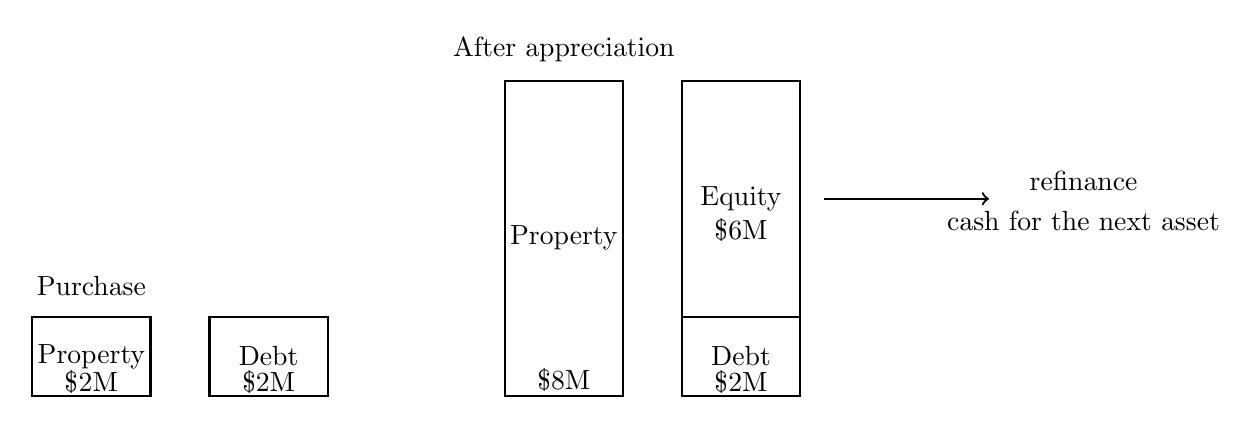
\begin{tikzpicture}[x=0.75cm,y=0.5cm]
\draw[thick] (0,0) rectangle (2,2);
\draw[thick] (3,0) rectangle (5,2);
\node at (1,2.8) {Purchase};
\node at (1,1) {Property};
\node at (1,0.35) {\$2M};
\node at (4,1) {Debt};
\node at (4,0.35) {\$2M};

\draw[thick] (8,0) rectangle (10,8);
\draw[thick] (11,0) rectangle (13,8);
\draw[thick] (11,2) -- (13,2);
\node at (9,8.8) {After appreciation};
\node at (9,4) {Property};
\node at (9,0.4) {\$8M};
\node at (12,1) {Debt};
\node at (12,0.35) {\$2M};
\node at (12,5) {Equity};
\node at (12,4.2) {\$6M};

\draw[->,thick] (13.4,5) -- (16.2,5);
\node at (17.8,5.45) {refinance};
\node at (17.8,4.45) {cash for the next asset};
\end{tikzpicture}
\end{figure}

The lecture also describes the refinance proceeds as tax free. We should preserve that as part of the speaker's claim, while also recognizing that the lecture does not supply a full tax derivation.

\section{Negotiation, structure, and buying access}

Once the leverage mechanism has been made explicit, the lecture turns back to the business side and asks about negotiation. The answer is again stripped of mystique: a deal has to work for both sides. If it works only for us, it will not last. If it works only for them, we have wasted our time. The lecture is not giving a game-theoretic model, but it is giving a symmetry condition: durability requires reciprocal value.

That symmetry reappears when the speaker is asked what people do wrong when they try to sell a company. His answer is structural. They have not built enough platform, process, and procedure to obtain the highest valuation. The company is therefore not only an income stream. It is also an organized object that a buyer must be able to read, trust, and scale.

The discussion of LLC formation, and the brief Busy promotion that follows, should be read in that light. The promotional material itself can be compressed, but the lecture's conceptual point is real: entity structure is not ornamental paperwork. It is the first layer of business foundation. The speaker even says that having the right structure is like getting dressed in the morning: it simply has to be done.

\subsection{Question \& Answer}

\paragraph{Question.}
Should we buy a business or start one?

\paragraph{Answer.}
The answer first sounds contradictory. The operator says ``start,'' even though he himself bought a business. The contradiction dissolves as soon as he explains what he actually purchased. He did not buy income. He bought access.

We may therefore schematize the distinction as follows:
\begin{align}
\text{buy} &\longrightarrow \text{access to industry} + \text{access to key employees},\\
\text{start} &\longrightarrow \text{build directly from tools, capital, and platform}.
\end{align}

This is one of the lecture's clearest ideas. Buying a business is not necessarily the purchase of a cash flow. It may be the purchase of position. We buy when we need entry, relationships, or people already in motion. We build when we already have the tools and want authorship of the machine from the ground up.

The lecture then resets sharply. We leave the food-distribution operator and go to a new scale marker altogether: John Ruiz and his compound.

\section{John Ruiz: a bigger platform, the same rules}

The John Ruiz segment begins theatrically. The host announces his forty-first billionaire interview and heads to what he insists is not merely an estate but a compound, valued at roughly \$175 million. The spectacle has a narrative purpose. Before Ruiz speaks about rules, platform, sacrifice, and execution, the lecture wants us to register the scale that those words are supposed to explain.

\paragraph{Anecdote.}
Ruiz gives an immigrant-start story in concentrated form. His father came from Cuba with five children and had been homeless. Ruiz was the first in the family to go to college, then to law school. He says he began with an \$800 Discover credit card, opened his own firm, and when he could not pay rent he paid in labor instead. In other words, before owning capital he rented position with effort.

\begin{align}
C_0 &= \$800,\\
V_{\text{home,now}} &\approx \$175 \times 10^6,\\
P_{\text{home}} &\approx \$46 \times 10^6.
\end{align}

The transcript then gives a garbled line about later improvements. If we normalize it cautiously as roughly another \$20 million of capital put into the house, we get only a provisional basis estimate:
\begin{align}
B &\approx P_{\text{home}} + I_{\text{capex}} \approx \$66 \times 10^6,\\
U &\approx V_{\text{home,now}} - B \approx \$109 \times 10^6.
\end{align}

\begin{remark}
The improvement figure is unstable in the transcript. The quantities \(B\) and \(U\) are therefore only rough bookkeeping devices, not settled profit calculations.
\end{remark}

\paragraph{Claim.}
Ruiz's central doctrinal statement is that it takes the same effort to make \$1 as to make \$100 million. We should not force that into a literal law. The point is heuristic. The rules are the same; the laws are the same; only the platform is bigger.

The host later compresses this into a ladder of problem classes:
\begin{equation}
\$1 \longrightarrow \$10^4 \longrightarrow \$10^6 \longrightarrow \$10^9.
\end{equation}

That ladder should be read as a map of scale, not as an equality of effort functions. The lecture's meaning is that the kinds of judgment required do not become magical at higher numbers. What changes is the size of the arena and the level of the players already inside it.

\paragraph{Mechanism.}
Ruiz makes this less mystical still. One does not have to reinvent the wheel. Innovation is a special case. Most of the time, one simply does the work on a larger platform, often with counterparties who already understand the game and move quickly.

\paragraph{Execution.}
The price of that platform, as he describes it, is availability and repetition rather than glamour:
\begin{align}
s &\in [3.5,4]\ \text{hours/night},\\
N_{\text{email}} &> 10^3/\text{day}.
\end{align}

He also says that his truly solid sleep may be closer to two hours. These are not prescriptions. They are evidence for how he wants the lecture to understand scale: not as display but as continued responsiveness. If people call and one does not respond, he says, it will not work. There is not one text message he does not read.

The interview then widens into a moral account of scale. What billionaires have in common, he says, is belief in themselves and a refusal to listen to noise. Money, for him, comes and goes; if he lost everything, he says he could sell lemons on a corner and come back. Criticism from the outside is explained as envy. His father's maxim gives the moral center of this section: there is no bad business with a good man, and no good business with a bad man.

Only after these character claims does Ruiz return to direct commercial advice. A negotiation succeeds when the other side understands why what we have is valuable to them, not to us. The section closes as it should close, not with the house but with repetition: it is not about what one does on a single inspired day. One has to do it every day. The goal is execution.

\subsection{Question \& Answer}

\paragraph{Question.}
Is entrepreneurship for everyone?

\paragraph{Answer.}
Ruiz's first answer is no. It takes dedication, hard work, sacrifice, and unusual availability. Later, when the same question is put to Jordan Belfort, the answer is reframed rather than reversed. Belfort says that not everyone needs to be an entrepreneur, but anyone who wants abundance, autonomy, and the ability to choose life on his own terms will find a paycheck a narrow path. Taken together, the lecture's answer is that entrepreneurship is not a universal duty. It is a route chosen by people whose desires are large enough, and whose tolerance for cost is high enough, to make the route necessary.

\section{Jordan Belfort: formula, persuasion, and qualification}

The final reset is to Jordan Belfort. The host arrives on Star Island with the now-explicit slogan that proximity is power and that the more hands one shakes, the more money one makes. That slogan is crude, but it is faithful to the structure of the lecture. We have moved from Miami as a money field to an access network within that field.

Belfort begins, characteristically, with a headline number:
\begin{align}
Y_{\text{day,cash}} &= \$23 \times 10^6,\\
r_{\text{cash}} &\approx \frac{\$23 \times 10^6}{4\ \text{min}} \approx \$5.75 \times 10^6/\text{min}.
\end{align}

The rate is only arithmetic on the anecdote, but it helps us see how the lecture is shifting focus. We are no longer primarily studying exits or houses. We are studying the communicative machinery that can organize people and capital at very high velocity.

\paragraph{Claim.}
Belfort insists that every entrepreneur is a salesperson. This is not because every entrepreneur must always be pitching a product. It is because the entrepreneur must sell a future. To recruit great employees, one must make them buy into a vision.

\paragraph{Mechanism.}
He describes the chain directly:
\begin{equation}
\text{vision} \longrightarrow \text{emotional connection} \longrightarrow \text{commitment} \longrightarrow \text{effort}.
\end{equation}

If the vision is strong but the explanation is weak, the enterprise still fails at the level of recruitment. People will then work only for compensation. They will not work for mission.

The lecture then moves from recruitment to the problem of how money-making capability is found in the first place. Belfort says the hardest part is finding a formula to make money. Once that formula is found, money comes hard and fast. His phrase that the only way to get rich is quickly is immediately qualified: he does not mean a get-rich-quick scheme. He means a long period of failed attempts, pivots, and alignment, followed by sudden acceleration once the elements finally click.

We may write that sequence, cautiously and only as a transcript-based reconstruction, as
\begin{equation}
\text{trial} \longrightarrow \text{pivot} \longrightarrow \text{fit} \longrightarrow \text{acceleration}.
\end{equation}

That is not Belfort's literal notation, but it is the logic he describes: one starts with a plan, discovers that it does not work the first time, keeps pivoting, and eventually finds the missing piece of the puzzle.

\subsection{Question \& Answer}

\paragraph{Question.}
How do we turn a no into a yes?

\paragraph{Answer.}
Belfort refuses the premise. A real salesperson does not try to force a genuine no into a yes. A true no ends the path. The real field of skill is the territory of hesitation: ``let me think about it,'' ``call me back,'' ``let me speak to my wife,'' ``let me talk to my business partner.''

The distinction may be written schematically as
\begin{equation}
\text{No} \longrightarrow \text{Exit},
\qquad
\text{Hesitation} \longrightarrow \text{Clarify need} \longrightarrow \text{Advance toward yes}.
\end{equation}

\begin{figure}
\centering
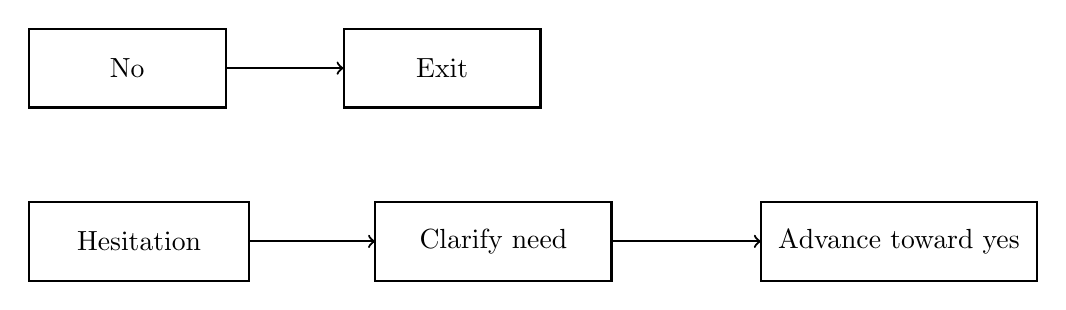
\begin{tikzpicture}[x=1cm,y=1cm]
\draw[thick] (0,0) rectangle (2.5,1);
\node at (1.25,0.5) {No};
\draw[->,thick] (2.5,0.5) -- (4,0.5);
\draw[thick] (4,0) rectangle (6.5,1);
\node at (5.25,0.5) {Exit};

\draw[thick] (0,-2.2) rectangle (2.8,-1.2);
\node at (1.4,-1.7) {Hesitation};
\draw[->,thick] (2.8,-1.7) -- (4.4,-1.7);
\draw[thick] (4.4,-2.2) rectangle (7.4,-1.2);
\node at (5.9,-1.7) {Clarify need};
\draw[->,thick] (7.4,-1.7) -- (9.3,-1.7);
\draw[thick] (9.3,-2.2) rectangle (12.8,-1.2);
\node at (11.05,-1.7) {Advance toward yes};
\end{tikzpicture}
\end{figure}

This prepares the final ``sell me this pen'' exchange. The standard failed answer is to begin immediately describing the pen. Belfort reverses the question. How could he sell the pen without first knowing whether the other person wants one? The opening move is therefore diagnostic, not performative.

The lecture then eases briefly away from sales mechanics and back into character. Asked whether money changes people, Belfort says that it is like alcohol: it amplifies but does not transform. Asked about the best advice he ever received, he recalls early sobriety and the discipline of returning attention to the present rather than living in regret. That sequence matters. The lecture wants persuasion to end not in manipulation, but in judgment.

We can now see why the pen question closes the interview. It is not there merely because it is famous. It crystallizes the whole section. The first task of selling is not eloquence. It is qualification. We do not waste time selling to people who do not need or want the thing in question.

\section{Summary}

The chapter unfolds the way the lecture unfolds: by advancing from access to mechanism. We begin in Miami as a field of concentrated wealth, watch several attempts fail, and only then arrive at the first real operator. From him we get an operating machine in miniature: products, procurement, sales coverage, pricing, and service organized well enough to turn a \$300{,}000 acquisition into repeated nine-figure exits.

From there the lecture opens a second machine. Real-estate appreciation is converted into usable capital by refinancing the equity created inside the asset rather than selling the asset itself. Ruiz then shifts the scale of the discussion. The rules do not change, he says; the platform changes. What follows from that larger platform is availability, self-belief, negotiation discipline, and daily execution. Belfort finally narrows everything down to the language of persuasion: vision, recruitment, pivoting until a formula works, distinguishing true refusal from mere hesitation, and qualifying demand before trying to close.

Even the video's closing turn back toward the School of Hard Knocks network belongs to the same logic. Access is not an ornament laid on top of business method. It is part of business method. Wealth, in this lecture, is built through position, structure, leverage, execution, and the disciplined search for the real yes.